\documentclass[10pt]{article}
\usepackage[polish]{babel}
\usepackage[utf8]{inputenc}
\usepackage[T1]{fontenc}
\usepackage{amsmath}
\usepackage{amsfonts}
\usepackage{amssymb}
\usepackage[version=4]{mhchem}
\usepackage{stmaryrd}
\usepackage{graphicx}
\usepackage[export]{adjustbox}
\graphicspath{ {./images/} }

\title{KLASY PO SZKOLE PODSTAWOWEJ }

\author{}
\date{}


\newcommand\Varangle{\mathop{{<\!\!\!\!\!\text{\small)}}\:}\nolimits}

\DeclareUnicodeCharacter{00D7}{\ifmmode\times\else{$\times$}\fi}

\begin{document}
\maketitle
\begin{enumerate}
  \item Pudełko na klocki ma kształt trójkąta równobocznego o boku \(a \mathrm{~cm}\). Pudełko jest szczelnie wypełnione przez \(2 n\) klocków, z których \(n\) jest w kształcie trójkąta równobocznego o boku 1 cm , a \(n\) - trójkąta równobocznego o boku 2 cm (jest jedna warstwa klocków). Jaka jest najmniejsza możliwa wartość \(a\) ?
  \item Średnica koła numer 1 wynosi 24 mm . Oblicz średnicę koła numer 2.
  \item Na planszy o wymiarach 9×9 gramy w statki. Każdy z graczy oprócz innych statków posiada pancernik reprezentowany przez prostokąt o\\
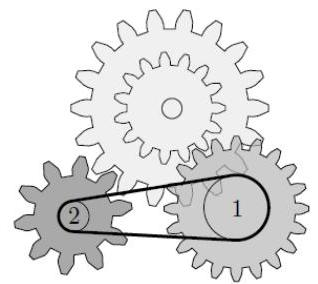
\includegraphics[max width=\textwidth, center]{2024_11_21_8959f10a7e6dd43271bbg-1}\\
wymiarach \(5 \times 1\) lub \(1 \times 5\). Jaką minimalną liczbę strzałów musimy oddać, by choć raz trafić pancernik, niezależnie od jego lokalizacji?
\end{enumerate}

\section*{KLASY PO GIMNAZJUM}
\begin{enumerate}
  \item Udowodnij, że dla dowolnych liczb dodatnich \(x, y\) prawdziwa jest nierówność
\end{enumerate}

\[
x^{4}+y^{4}>x y^{3}
\]

\begin{enumerate}
  \setcounter{enumi}{1}
  \item W trójkącie ostrokątnym \(A B C \Varangle A C B=60^{\circ}\). Punkty \(P\) i \(Q\) są rzutami prostokątnymi odpowiednio punktów \(A\) i \(B\) na proste \(B C\) i \(A C\). Punkt \(M\) jest środkiem boku \(A B\). Udowodnij, ze trójkąt PMQ jest równoboczny.
  \item Na pewnej wyspie żyją trzy rodziny. Do każdej z nich należy dwóch synów i dwie córki. Na ile sposobów można zaaranżować sześć małżeństw (kobieta + mężczyzna) pomiędzy tymi osobami, zakładając, że małżeństwa pomiędzy rodzeństwem są zabronione.
\end{enumerate}

\end{document}